\chapter{Lois de comportement}
\section{Problèmes dynamiques et quasi-statiques}
Pour résoudre un problème de Mécanique des Solides, il faut calculer la solution $(u_i, \sigma_{ij})$, c'est à dire calculer les champs de vecteurs déplacements $u_i(x)$ et de tenseurs des contraintes $\sigma_{ij}(x)$, à partir des données, qui sont constituées par
\begin{enumerate}
    \item L'ensemble des sollicitations imposées au solide
        \begin{itemize}
            \item forces volumiques
            \item conditions aux limites (forces ou déplacements imposés à la surface).
        \end{itemize}
    \item Les conditions initiales, précisant la position et la vitesse initiale du solide.
\end{enumerate}
\textbf{Exemple:} Réservoir sphérique soumis à une pression intérieure $n$
\begin{center}
    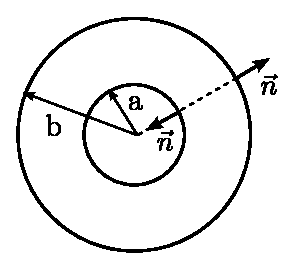
\includegraphics{../images/T1_Ch04-0001}
\end{center}
\begin{itemize}
    \item Les forces volumiques sont supposées nulles (pesanteur négligeable)
        \begin{equation}
            f_i = 0
            \label{eq:Ch04-001}
        \end{equation}
    \item La surface extérieure $r=b$ est soumise à la pression atmosphérique, la contrainte est donc nulle d'après \eqref{eq:Ch02-002}:
        \begin{equation}
            r=b \text{ : } \sigma_{ij} n_j = T_i = 0
            \label{eq:Ch04-002}
        \end{equation}
    \item La surface intérieure $r=a$ est soumise à la pression $p$ (supposée mesurée par rapport à la pression atmosphérique) d'où
        \begin{equation}
            r=a \text{ : } \sigma_{ij} n_j = T_i = -p n_i
            \label{eq:Ch04-003}
        \end{equation}
\end{itemize}
\begin{enumerate}%[a)] FIXME
    \item Problème dynamique:  On  donne  la pression  $p(t)$  comme  fonction  du  temps; on  donne  également les  conditions  initiales  -- par  exemple,  à  $t=0$,  le réservoir est au repos
        \begin{equation}
            u_i(x,0)=0 \quad V_i(x,0) = \frac{\partial u_i}{\partial t}(x,0) = 0
            \label{eq:Ch04-004}
        \end{equation}
        et on cherche la solution $u_i(x,t),\ \sigma_{ij}(x,t)$ qm doit vérifier l'équation du mouvement \eqref{eq:Ch03-028}
        \begin{equation}
            \rho_0 \frac{\partial^2 u_i}{\partial t^2} = \frac{\partial \sigma_{ij}}{\partial x_j} + f_i
            \label{eq:Ch04-005}
        \end{equation}
        avec \eqref{eq:Ch04-001}, les conditions aux limites \eqref{eq:Ch04-002} et \eqref{eq:Ch04-003}, et les conditions initiales \eqref{eq:Ch04-004}.
        Ce problème correspond par exemple à l'étude de la mise en charge brutale du réservoir.
        Moyennant une modification des conditions initiales \eqref{eq:Ch04-004}, il correspond aussi à l'étude des vibrations du réservoir, si l'on impose une pression $p(t)$ sinusoïdale
        \begin{equation}
            p(t) = p_0 \cos \omega t
            \label{eq:Ch04-006}
        \end{equation}
        on recherche alors une solution périodique en $t$, condition qui remplace \eqref{eq:Ch04-004}.
    \item Problème statique: La pression $p$ est constante c'est la pression en service du réservoir.
        On recherche alros une solution statique, c'est à dire indépendante du temps $u_i(x),\ \sigma_{ij}(x)$ vérifiant les équations d'équilibre
        \begin{equation}
            \frac{\partial \sigma_{ij}}{\partial x_j} +f_i = 0
            \label{eq:Ch04-007}
        \end{equation}
        avec \eqref{eq:Ch04-001} et les CI (conditions aux limites) \eqref{eq:Ch04-002} et \eqref{eq:Ch04-003}.
        Le temps a disparu, et les conditions initiales n'ont plus lieu d'être.
    \item Problème quasi-statique: On suppose comme en a) que la pression $t$ varie au cours du temps, $p(t)$, mais on fait l'hypothèse suivante
        \par\underline{Hypothèse quasi-statique:} Les évolutions sont suffisamment lentes pour que, dans l'équation du mouvement \eqref{eq:Ch04-005}, on puisse négliger le terme d'accélération et donc la remplacer par l'équation d'équilibre \eqref{eq:Ch04-007}.

        En d'autres termes, la sollicitation dépend du temps, mais on résoud à chaque instant un problème statique.
        Cette hypothèse est tout à fait essentielle en mécanique des solides, car elle permet de ramener à des problèmes statiques les problèmes réels qui, eux, dépendent toujours du temps.
        L'essentiel de ce cours sera désormais limité au cas où cette hypothèse est valable, l'étude des problèmes réellement dynamiques (chocs, vibrations) étant renvoyée au cours de Mécanique des Vibrations.
\end{enumerate}
\section{Conditions aux limites}
\textbf{Exemple 2.} Ecrasement d'un lopin entre les deux plateaux rigides d'une presse:
\begin{wrapfigure}{l}{7cm}
    \begin{center}
        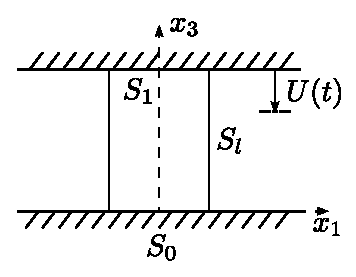
\includegraphics{../images/T1_Ch04-0002}
    \end{center}
\end{wrapfigure}
Un bloc métallique cylindrique est écrasé entre les deux plateaux rigides d'une presse.
Le plateau inférieur $x_3 =0$ est immobile, tandis que le plateau supérieur $x_3 =h$ s'enfonce d'une longueur $U(t)$.
À nouveau, on peut s'intéresser aux problèmes dynamique, statique ou quasi-statique, mais nous nous limiterons au dernier cas: la solution dépend du temps puisque la sollicitation en dépend, mais nous écrirons néanmoins les équations d'équilibre.

Comme dans l'exemple précédent, et comme dans la majorité des cas en Mécanique des Solides, la seule force de volume est la pesanteur, et nous la négligerons, d'où \eqref{eq:Ch04-001}.
La surface latérale $S_l$ est libre de contraintes
\begin{equation}
    \text{sur } S_l:\quad T_i = \sigma_{ij} n_j = 0
    \label{eq:Ch04-008}
\end{equation}
Sur les extrémités $S_0$ $(x_3=0)$ et $S_1$ $(x_3=h)$, la condition exprimant la rigidité des plateaux porte sur le déplacement vertical
\begin{equation}
    \begin{cases}
        x_3 = 0: & u_3 = 0 \\
        x_3 = h: & u_3 = -U(t)
    \end{cases}
    \label{eq:Ch04-009}
\end{equation}
mais les autres conditions aux limites dépendent des conditions de contact entre les plateaux et le lopin.

\emph{S'il n'y a pas de frottement}, c'est à dire si le contact est parfaitement lubrifié, alors la force de contact, en $x_3=h$, par
\begin{equation}
    \vec{n} = \left( 0,0,+1 \right), \quad \vec{T} = \left( \sigma_{13}, \sigma_{23}, \sigma_{33} \right)
    \label{eq:Ch04-010}
\end{equation}
doit être normale à la surface de contact.
Les conditions \eqref{eq:Ch04-009} doivent être complétées par les conditions $\sigma_{13} = \sigma_{23} = 0$
\begin{equation}
    \left\{
    \begin{aligned}
        x_3 = 0: & u_3 = 0, & \sigma_{13} = \sigma_{23} = 0 \\
        x_3 = h: & u_3 = -U(t), & \sigma_{13} = \sigma_{23} = 0
    \end{aligned}
    \right.
    \label{eq:Ch04-011}
\end{equation}

\emph{S'il n'y a pas de glissement}, c'est à dire s'il y a adhérence complète entre le lopin et le plateau, alors il faut compléter \eqref{eq:Ch04-009} par les conditions cinématiques d'adhérence $u_1 = u_2 = 0$
\begin{equation}
    \begin{cases}
        x_3 = 0: & u_1 = u_2 = u_3 = 0 \\
        x_3 = h: & u_1 = u_2 = 0, u_3 = -U(t)
    \end{cases}
    \label{eq:Ch04-012}
\end{equation}

Dans le cas réel, il y a frottement entre le plateau et le lopin, et il faut compléter \eqref{eq:Ch04-009} par la condition exprimant la loi de frottement. 
Nous adoptons la loi de frottement de Coulomb, avec un coefficient de frottement $f$,
\begin{equation}
    \left\{
    \begin{aligned}
        \vec{V} = 0 & \text{si} & |\vec{T}| < fN \\
        \vec{V} = \lambda \vec{T} & \text{si} & |\vec{T}| = fN, \lambda \geq 0
    \end{aligned}
    \right.
    \label{eq:Ch04-013}
\end{equation}
\begin{wrapfigure}{r}{4cm}
    \begin{center}
        \includegraphics{../images/T1_Ch04-0003}
    \end{center}
\end{wrapfigure}

que l'on peut encore rééecrire sous la forme
\begin{equation}
    \left\{
    \begin{aligned}
        \vec{V} = \lambda \vec{T}\\
        \lambda \geq 0, \quad fN - |\vec{T}| \geq 0, \quad \lambda \left( fN - |\vec{T}| \right) = 0
    \end{aligned}\right.
    \label{eq:Ch04-014}
\end{equation}
On obtient alors
\begin{equation}
    \left\{
    \begin{aligned}
        x_3 = 0:&\quad u_3 = 0, \frac{\partial u_1}{\partial t} =\lambda \sigma_{13}, \frac{\partial u_2}{\partial t} = \lambda \sigma_{23}, \\
            & \lambda \geq 0, -f \sigma_{33} - \sqrt{\sigma_{13}^2 + \sigma_{23}^2} \geq 0, \lambda \left( -f \sigma_{33} - \sqrt{\sigma_{13}^2 + \sigma_{23}^2} \right) = 0 \\
        x_3 = h:&\quad u_3 = -U(t), \frac{\partial u_1}{\partial t} = -\lambda \sigma_{13}, \text{etc.}
    \end{aligned}
    \right.
    \label{eq:Ch04-015}
\end{equation}

Le problème de l'écrasement d'un lopin consiste donc à trouver $u_i(x,t), \sigma_{ij}(x,t)$, vérifiant à chaque instant les équations d'équilibre \eqref{eq:Ch04-007} avec $f_i = 0$, et les conditions aux limites \eqref{eq:Ch04-008} et \eqref{eq:Ch04-011}, \eqref{eq:Ch04-012} ou \eqref{eq:Ch04-013}, suivant la nature du problème et suivant la précision des résultats cherchés: le problème \eqref{eq:Ch04-015} est certainement plus proche de la réalité que les problèmes \eqref{eq:Ch04-011} ou \eqref{eq:Ch04-012}, mais les problèmes \eqref{eq:Ch04-011} et \eqref{eq:Ch04-012} sont beaucoup plus simples, et peuvent constituer une approximation suffisante pour les besoins que l'on a.
De même, si le frottement est important, le problème \eqref{eq:Ch04-012} est certainement plus proche de la réalité qUe le problème \eqref{eq:Ch04-011}.
Néanmoins, le problème \eqref{eq:Ch04-011}, qui, comme on le verra, se résoud très simplement, peut être un approxmation suffisante, par exemple pour le calcul de la force $F$ à appliquer sur la presse et qui sera donnée par
\begin{equation}
    F(t) = - \iint_{S_0} \sigma_{33} \ud x_1 \ud x_2 = - \iint_{s_1} \sigma_{33} \ud x_1 \ud x_2
    \label{eq:Ch04-016}
\end{equation}

\textbf{Exemple 3.} Bloc pesant posé sur un plan rigide.

\begin{wrapfigure}{l}{4cm}
\begin{center}
    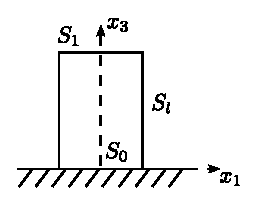
\includegraphics{../images/T1_Ch04-0004}
\end{center}
\end{wrapfigure}
Le bloc est soumis à la seule action de la pesanteur.
En notant $\rho_0 = \rho$ la masse volumique du solide, et $g$ l'accélération de la pesanteur, on a donc
\begin{equation}
    f_1 = f_2 = 0, \quad f_3 = -\rho g
    \label{eq:Ch04-017}
\end{equation}
La surface latérale $S_l$ et l'extrémité $S_1\ (x_3=h)$ sont libres de contraintes
\begin{equation}
    \left\{
    \begin{aligned}
        \text{sur } S_l & \sigma_{ij} n_j = 0 \\
        x_3 = h & \sigma_{13} = \sigma_{23} = \sigma_{33} = 0
    \end{aligned}
    \right.
    \label{eq:Ch04-018}
\end{equation}
Sur l'extrémité $S_0\ (x_3=O),$ les conditions aux limites dépendent, comme dans le cas précédent, des conditions de contact: dans le cas de non frottement on a
\begin{equation}
    x_3 = 0: \quad u_3 = 0 \quad \sigma_{13} = \sigma_{23} = 0
    \label{eq:Ch04-019}
\end{equation}
dans le cas de non glissement, on a 
\begin{equation}
    x_3 = 0: \quad u_1 = u_2 = u_3 = 0
    \label{eq:Ch04-020}
\end{equation}

\begin{wrapfigure}{l}{5cm}
    \begin{center}
        \includegraphics{../images/T1_Ch04-0005}
    \end{center}
\end{wrapfigure}
dans le cas du frottement coulombien, on a une expresslon analogue à \eqref{eq:Ch04-015}.
Toutes ces conditions supposent que le contact entre le bloc et le plan reste maintenu.
Il peut arriver -- figure ci-contre -- qu'une partie du bloc se soulève.
Il s'agit alors d'une liaison unilatérale.
La surface $S_0$ se décompose en deux zones (que l'on ne connaît pas, leur détemination fait partie du problème)
\begin{itemize}
    \item une zone de contact où l'on a
        \begin{equation}
            u_3 = 0, \quad \sigma_{33} \leq 0
            \label{eq:Ch04-021}
        \end{equation}
    \item une zone de non contact, libre de contraintes, où l'on a
        \begin{equation}
            u_3 \geq 0, \quad \sigma_{33} = 0
            \label{eq:Ch04-022}
        \end{equation}
\end{itemize}
On peut regrouper \eqref{eq:Ch04-021}, \eqref{eq:Ch04-022} en
\begin{equation}
    u_3 \geq 0, \quad \sigma_{33} \leq 0, \quad u_3 \sigma_{33} = 0
    \label{eq:Ch04-023}
\end{equation}
En supposant le contact sans frottement, il faut donc remplacer \eqref{eq:Ch04-019} par
\begin{equation}
    x_3 = 0 
    \begin{cases}
        \sigma_{13} = \sigma_{23} = 0 \\
        u_3 \geq 0, \quad \sigma_{33} \leq 0, \quad u_3 \sigma_{33} = 0
    \end{cases}
    \label{eq:Ch04-024}
\end{equation}

En toute rigueur, il aurait aussi fallu envisager cette possibilité dans l'exemple précédent, mais elle était peu plausible physiquement.

On pourrait également envisager d'autres types de conditions aux limites sur $S_0$.
\begin{wrapfigure}{l}{3cm}
    \begin{center}
        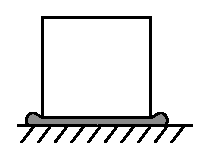
\includegraphics{../images/T1_Ch04-0006}
    \end{center}
\end{wrapfigure}
Par exemple, on peut imaginer de poser le bloc sur le plan par l'intermédiaire d'un ballon de baudruche contenant un gaz à la pression $p$.
Les efforts exercés sur le solide par le ballon se ramènent alors à une pression hydrostatique
\begin{equation}
    x_3 = 0: \quad \sigma_{33} =-p, \sigma_{13} = \sigma_{23} = 0
    \label{eq:Ch04-025}
\end{equation}

On peut déterminer $p$ en remarquant que, d'après les équations d'équilibre, les efforts exercés sur le bloc à travers $S_0$ doivent équili­brer les autres efforts appliqués, c'est à dire en l'occurence le poids du bloc.
On obtient donc la condition suivante
\begin{equation}
    -\iint_{S_0} \sigma_{33} \ud x_1 \ud x_2 = \rho g S h
    \label{eq:Ch04-026}
\end{equation}
valable quelles que soient les conditions aux limites sur $S_0$.
Avec les conditions \eqref{eq:Ch04-025}, on en tire la valeur de $p$
\begin{equation}
    p = \rho g h
    \label{eq:Ch04-027}
\end{equation}

De manière générale, dans un problème réel, l'écriture des conditions aux limites est une étape tout à fait essentielle, car d'une part ces conditions comprennent l'essentiel de la physique du problème, d'autre part elles conditionnent la facilité -- voire la possibilité -- de la résolution du problème mathématique obtenu.
Il faudra souvent faire un compromis entre la précision de la description physique et la facilité de résolution du problème mathématique.

\section{Lois de comportement}
\endinput
Pour résoudrE: un problème de Déc.;.:::'::.;,.; àes scl::2s, _c._~ CODe résoudre un systêc~ d'€quations aux ~érivéeE ;Er~ielles. =2ur :'i~s:a~t, nous avons trois équations scalaires -les ÉC:t.,;.ations du J:}uve=ent (5) ou les équations d'équilibre (7), suivant que l'en considère le Froblè=2 dyna­mique DU le problème qt!.asi-~t2.t.icp.!e -FC"'.!!" 9 Ch2~pS ~:1co:1nus: 3 co:::pcsantes du déplacement ..u.4 C'x.,-t) et 6 composantes du tenseur des contraintes cr;,,~ ('-x.I.c~­Il manque donc 6 équations scalaires. Ces 6 équations nous seront fournies par la "loi de comportement" du matériau. Tout'es les équations écrites jus­qu'à présent. é-taie-nt. -dans. le cadIe-d··' une-· schématisation donnée -univeI­selles, càd indépendantes du matériau considéré. Les équations écrites au § 1.2 restent les mêmes pour un bloc d'acier, d'aluminium, de matière plas­tique, de caoutchouc, de bois, de béton,' d'argile, de pâte à modeler, etc ... , sous la seule réserve que les hypothèses fondamentales soient vérifiées (théorie du premier gradient, petites déformations). 
De manière générale, la loi de comportement se présente comme une "relation" entre le tenseur des contraintes et le tenseur des déformations. Cette relation peut être de nature très diverse -nous en verrons quelques exemples au § 2 -mais elle sera en général de nature "fonctionnellel1. A 
quelques cas singuliers près, nous pouvons admettre qu'elle donne le tenseur des contraintes à partir de l'histoire du tenseur des déformations -càd de la valeur du tenseur des d~forrnations à l'instant considérê et à tous les 1n5-­
tants antérieurs -ou bien le tenseur des déforrrœtions à partir de l'histoire du tenseur des contraintes. 

.. 
(28) 
Ht) = [ t(J(k-A)) 
hO 
Cette loi de comportement ne peut être déterminée qu'expérimentale­ment par un certain nombre "d'essais". Les essais les plus faciles à inter­préter sont les flessais homogènes" où l'on cherche à réaliser dans une éprou­vette un état de contrainte et de déformation homogène. L'exemple le plus simple est l'essai de compression simple, qui correspond à l'exemple 2 du § 1.2 . Si l'on cherche un état de contrainte et de déformation homogène 

alors la condition aux limites (8) sur la surface latérale montre que toutes les composantes de Cf';'6 l.t) sont nulles, sauf <T-en effet, sur St 1'1'\" =0
n 
tanèÏs que 'TI.~ et 'TI.~ sont quelconques -et (16) donne C-,; (.t) = -F;,t) ,'5 
0 0 0 (3e, (]):) 
0 0 0= 
l 
Lo c -F(:t)jS J 
rie ccnportement (28) donne alors &: (, k'1 en fonction dE: • Oc 0:­tien~ alors la forme générale GU déplacement par (III.62) 
r JJ... = E.~~ ':1:, ... E,,, 'X.:, .,. ~1;:I:.~ + W~"X.~ w. X~ T c.
-
(31 ) ...
~ JJ..~ = E~l, ':1:, + El.l, :L~ + ~~ô X. T W; 'X.. -w1 -:c. c,..
, 
_ w 

~
( JJ..~ = E~; :1:.. ;-~J,; XJ. + En 'X.. + Cù1'X.~ :, . T .c. 
La CL (9) en x =0 donne alors
3 

La CL (9) en x=h est alors vérifiée si
3
(32) et il vient 

.A.l..{':I:,..t:) .,. EH 'X.~ ;-(f..2. 'XL T t E.1; 'X~.
-w.) 
(33) .A.l.:z, (lX,l) = (!:~~ +-W~) 'X.. + f:z,l. 'l:~ +-2, E:z,; 'X; 
r Al. (IX)k) = -U(t) IX../Yn, 
Et la solution définie par (30) , (33) est solution du problème associé au cas sans frottement défini par les CL (II). Ainsi, pour réaliser un essa~ de compression simple, on écrase un lopin en lubrifiant le contact, pour s'approcher au rnaXlmurn des conditions de non frottement, et en imposant, par exemple, une force F(k) -essai à force imposée -, la mesure des dépla­cements donne alors !(k) , et permet donc de déterminer la loi de compor­tement pour un tenseur cr de la forme (30). 
Si le matériau est isotrope -notion que nous préciserons plus tard -alors un tenseur cr("\:) de la forme (30) produit une déformation de la forme 
(34) w:) 

La déformation se réduit à un écrasement longitudinal, mesuré par UC.\;) 
et une dila ta tian transversale que l'on mesure fac ilement à l t aide dl une 
jauge de déformation. 
1.4 LES ESSAIS 	CLASSIQUES 
L'essai de COffipreSSlon simple est le protoc)pe ries essais homo­gÈnes. L'idée de base est de réaliser un état àe contrainte et è2 déforma­tion hOTIXJgène qui peut alors être déterminé par des mesures glo::ales cl' ef­forts et de déformation. Pour les métaux et la plupart des soliàes, l'essai de base est "l'essai de traction", oU un barreau cylindrique de longueur i et de secticn S est SOU~lS à une force 18~gitudi~ale F . L'état de ~8~­trainte et de déformation a la même forme (30), (34) que pour l'essai de compression. 
F 
':tA On mesure -la force de trac tian FU;) -l'allongement longitudinal 


-l'allongement transversal ET (t) 
F 
ir F(J;)/S o 
(35) 
dl"" = 0 	o 
o

L 0 



Les conditions aux limites (11) de non frottement sont pratiquement irréali­sables, mais on constate expérimentalement que, pourvu que l'éprouvette soit 
assez longue, alors les résultats de l'essai ne dépendent pratiquement pas 
de la manière dont est appliquée la force f , càd des conditions aux limi­
t~s précises sur So et 51 • C'est le principe de Saint-Venant, sur lequel 
nous reviendrons au chapitre VII. 
L'essai de traction est le plus simple à réaliser, mais il ne per­met d'obtenir la loi de comportement que pour un tenseur des contraintes de 
traction ou compression simple. Cela suffit pour déterminer complètement cer­
taines lois de comportement, mais il est souvent nécessaire de réaliser des états de contrainte plus complexes.Le choix est alors guidé par la possibili­té technologique de réaliser un état de contrainte et déformation le plus ho­mogène possible. L'essai le plus couramment utilisé pour les métaux est l'es­sai de "traction-torsion" d'un tube mince. Un tube mince de diamètre D, d'é-
F 

paisseur ..e. et de longueur .c est soumis à 
,­
une force longitudinale F(k; ~3 et à un couple 
de torsion 

On mesure 
, ,nl,'-),If

-1 allongement longitudinal u~~ ~ l'allongement transversal < r..t'
c. i \. , -la rotation relative tJ.e(x) des deux sections 
extrémi tés. tw~e sc:t suffisamoent ~ince, l'état de contrainte et ceIO=~­

~
tian est G2tr...nê àans le repère local (~'l..'.e.@, .e~) associé aux coorcionnées cy­

; 1 [> ,
0 0 0 0 
1 rET 
<-1 1 
(36) cr 0 0 iM/rrli e i &: 1 0 }) t:.fj/4 t • 
= ET
=1 
, i 
L 1 0 J L , ,
tMjrr n".e-FI Tf. Ti~ l 0 :Dtle/4-L M./L 
superposition d'une traction simple et d'un cisaillement simple. 
Ce type dtessai convient pour des matériaux suffisamment consistants_ En mécanique des sols, où l'on a affaire à des matériaux peu ou pas cohérents, on utilise classiquement deux types d'essais. 

Dans l'essai oediométrique, on comprlme le matériau dans un moule rigide. On réalise ainsi un état de contrainte et de déformation de la forme 

o 
(37) 
o o 



Dans l'essai "triaxial", on place une éprou­vette dans une cellule triaxiale que l'on sou­
p 
met à une pression ""fL et on superpose une, force longitudinale P On réalise ainsi un état de contrainte et de déformation de révolution (§ II.I.3) 

o 

o o 
(38) 
o o o o 
qr =
o 
Tous ces essaIS homogènes présentent l'avantage de pouvoIr s'inter­préter directement en termes de loi de comportement. Mis à part l'essai de traction, ils présentent cependant l'inconvénient d'être assez fins, nécessi­tant de grandes précautions pour obtenir des résultats significatifs. Dans la pratique courante, on utilise souvent des essais non homogènes, souvent issus de la tradition (essai pénétrornétrique en Mécanique des Sols, essai de dureté ou de résilience pour les métaux) qui permettent d'obtenir simplement des ca­ractéristiques globales du comportement. Malheureusement, ces essalS ne four­nissent sur les lois de comportement que des informations qualitatives, que l'on ne peut pas utiliser directement. 
2. COMPORTEMENT DES SOLIDES 
=========================== 
2.1 DIVERSITE DES COMPORTEMENTS 
Le but de ce paragraphe est double: d'une part nOUS allons décrire quelques uns des types de comportement que l'on peut rencontrer; d'autre part nous allons introduire la terminologie utilisée pour caractériser ces compor­tements. 
Pour les métaux à température ambiante, le comportement est convena­blement décrit par la courbe de traction, résultat de l'essai de traction. On fait croître la force F et on mesure l'allongement longitudinal 
13 
c. 
Aciers durs, métaux non ferreux
Acier doux 
-59 ­
La courbe se divise en trois régions. La région DA correspond à un comporte­
ment élastique linéaire, dont les deux caractéristiques essentielles sont: 
a) réversibilité: si, arrivé au point ~ on diminue la contrainte, on re­
descend suivant la même courbe; 
b) linéarité: la contrainte est proportionnelle à la déformation. 
Cette région correspond à la déformation réversible du réseau cristallin. 

A partir du seuil A, on entre dans la zone AB de comportement plastique, essentiellement caractérisé par son irréversibilité: si, arrivé en b on décharge, alors on redescend, non pas le long de la courbe de char­ge b A, mais sur une droite b,<,. parallèle à GA. En fait le comportement est alors à nouveau élastique tant que l'on ne redépasse pas le nouveau seuil 
b. En particulier, on constate que la déformation plastique entre A et b a eu comme effet d'élargir la région élastique. C'est le phénom~ne d'écrouÏs­sage. 
Le point B correspond à l'apparit~on de la striction instabilité géométrique qui conduit à la localisation de la déformation -. La contrainte cr diminue alors jusqu'à rupture. En fait, il s'agit de la contrainte appa­rente, càd ramenée à la surface initiale, la contrainte vraie, càd ramenée à la surface réelle de la striction, elle, continue à augmenter. De toute façon, la déformation n'est plus homogène, et cette portion de courbe ne décrit pas directement le comportement. De plus, l'hypothèse des petites dé­formations n'est plus vérifiée. 
0. 

Matériaux fragiles 
Y----------~ f L 
[0' 

En compression simple, on obtient en général un comportement symétrique DA'B' 
(mais sans striction). Pour certains matériaux fragiles (béton, fonte, roches, etc ...), cependant, on obtient en compression simple un comportement ductile, comme celui que nous avons décrit, et en traction simple, un comportement fragile conduisant à rupture très rapide. Pour les métaux·, on observe souvent l'effet Bauschinger: après une précharge OAa.. en traction, l'écrouissage qUI se traduit par une augmentation du seuil en traction, entraîne également une 
diminution du seuil en compression, alors qu'au départ les deux étaient approximativement égaux. La courbe de traction permet également de décrire le comportement d'autres matériaux, comme le caoutchouc, (comportement élastique non linéaire en première approximation) ou les sols -on représente alors I-e résultat 
cr 


caoutchouc sols 
cl 1 un essai "triaxial" à 1-fixé -qui présentent un comportement de type 
élasta-plastique avec une régibn élastique très réduite et avec ou sans plC 
suivant que le matLriau est initialement plus ou ~ins tassé. 
Pour des matériaux comme les matières plastiques ou les métaux à haute température, la courbe de traction perd toute signification, car elle dépend de manière cruciale de la vitesse de déformation. On caractérise alors le comportement par des essais de fluage et de relaxation. Pour l'essai de fluage, toujours en traction ou compression simple, on impose une contrainte constante et on observe la déformation en fonction du temps: l'application 
----­

~rance 
instantanée 
rec. différée 
déf. 
instant dU. résiduelle 

------~--------------~t 

t 
Marériau de type fluide Solide 
de la contrainte s'accompagne d'une déformation instantanée, puis la déforma­tion se poursuit, puis se stabilise, soit vers une constante, soit vers un état de fluage stationnaire à vitesse de déforr,ation constante. Si à un lns­tant to on relache la contrainte, alors la d~f0rn3tion de d&compose en trois port Lt·S: 
-une d('formation instant3nt:"·c (rcc,t.nJ\'rance ins l:-4!1tanéé), 
-une d~f(\rmation obtenue rn)lre.ssÎvCr:Jént (Y"~LOUV'r3nce différé:c), 
-une déformation résiduelle qui subsiste, cette dernière pouvant disparaître pour un matériau de type solide. 
L'essai de relaxation consiste à appliquer une déformation constant,­et à observer la contrainte nécessaire 

Fluide Solide Si l'on pousse plus loin l'essai de fluage, on voit apparaître 

l fluage primaire II fluage secondaire III fluage tertiaire 
t 
après le fluage primaire (régime transitoire) et le fluage secondaire (régime stabilisé) une zone de fluage tertiaire qui correspond au phénomène I!d'endom­rnagementll (détérioration du matériau qui conduit à la rupture). 
Ce type de comportement dépendant du temps est appelé I!viscoplasti­que l1 ou "viscoélastiquefl , selon qu'il existe ou non un seuil en dessous du­quel le comportement peut être considéré comme élastique. En première appro­ximation, les matières plastiques ont un comportement viscoélastique, et les métaux à haute température un comportement viscoplastique. 
2. 2 HODELES RHEOLOGIQUES 
Il est important de savoir construire des modèles mathématiques de comportement décrivant, au moins qualitativement, les différents types de COlT"­portement que nous venons de présenter. Les modèles rhéologiques forment une classe déjà très vaste de tels modèles. Ils s'obtiennent par combinaison de 3 modèles élémentaires 
le ressort, modèle de C(lmportement élastique 
(39) cr = Et 

-62 ­-le patin, modèle de comportement plastique 
L = 0 si \cr 1< (To 
(40) E. > 0 Si cr 
=cro
[ . 

E. < 0 Si (J = -Uo 
l' amortisseur, modèle de comportement visqueux 
'7
. 
(41 ) (J E.
= ") • TI D 
Les modèles rhéologiques s'obtiennent par montage en parallèle (les contrain­
tes s'additionnent, les deformations sont les mêmes) ou en série (les défor­
mations s'additionnent, les contraintes sont les mêmes). 
Le comportement viscoélastique peut être représenté par une combi­naison de ressorts et d'amortisseurs . 
• Par montage en série d'un ressort et d'un amortisseur, OR obtient le modèle de Maxwell: 
. 
E
cr = EL, = '7 E.J., '7. 
(42) 
{ = E
[ , + EJ., 
CVW.l~ 
L.,
ou en éliminant El.
E, et El, 
cr cr
(43 ) E 
= + 
E 
"l 
qui est la loi de comportement sous forme différentielle. Conformément à (28) 
on voit que, connaissant 1 'histoire de 0-(ou de E. ), on peut en déduire la valeur à l'instant t de E (ou de cr par intégration de l'équation dif­férentielle (43) . 
• Par montage en parallèle d'un ressort et d'un amortisseur, on obtient le 
modèle de Kelvin-Voigt 
(44) 


__ Par montage en série-d'un modèle de-Maxwell et d'un modèle de Kelvin-Voigt, on obtient le modèle de Burgers 
(45) 
[ 


En éliminant E" E.l, et E?, , il vient 
" E3 .. .. [;:;
+ _~_+_,._ CT
+ = (E 1r +
( 46) E E CT -1 CT 
"l3 E, "l:l E, "1 ,. '1:. (\,"1') 
forme différentielle de la loi de comportement. En particulier, on obtient 


en fluage' une courbe qUI représente qualitativement le comportement de certaines matières plastiques. 
L---------------~t 
Et ainsi de suite. 
Les comportements élasto-plastiques s'obtiennent par combinaison de ressorts et de patins . 
• Par montage en série d'un ressort et d'un patin, on obtient un modèle 
élasta-plastique sans écrouissage 


• On obtient un modèle avec écrouissage linéaire montage suivant 

Enfin, on peut obtenir des comportements viscoplastiques par des combinaisons des trois éléments de base. Par exemple le modèle de Bingham 

permet de décrire le comportement du goudron et de certaines pâtes. 
De manière générale, le choix d'un modèle représentant le compor­tement d'un matériau réel est un problème difficile. Le comportement des matériaux réels est complexe, et nous n'en avons présenté qu'une esquisse 
très  incomplète.  Même  pour  des  matériaux aussi  courants  que  l'acier,  de  
nombreux  aspects  du  comportement  restent mal  connus,  et  il  est  impossible  
de  construire  un  modèle .représentant  le comportement  d'un rnatérjau donné  

en toutes circonstances. Dans chaque problème, il convient de choisir le modèle le plus simple conduisant à des résultats satisfaisants pour l'uti­
lisation qu'on veut en faire. Dans certains cas, en particulier si l'on recherche une grande fiabilité, il conviendra de faire le calcul avec une loi de comportement très sophistiquée, prenant en compte tous les risques de ruine possibles, ceS calculs étant rendus possibles par les développe­ments de l'informatique. Dans d'autres cas, par contre, on pourra se satis­faire d'approximations plus grossières du comportement, et c'est la raison d'être des modèles élémentaires qui feront l'objet de la suite de ce cours. 
-65 ­Chapitre V 

